\section{Overview}\label{sec:overview}

% \begin{figure}
  \begin{subfigure}[c]{\columnwidth}
  \[
    \arraycolsep=3pt\begin{array}{rlrl}
        \text{pattern term} & \spat & ::= &
          \term{\ophole} ~\vert~
          \term{\svar{x}} ~\vert~
          \term{\sparen{\spat}} \\
        & & \vert &
          \term{\spat~\binhole~\spat} ~\vert~
          \term{\sprod{\spat}{\spat}} \\
        \text{expression term} & \sexp & ::= &
          \term{\ophole} ~\vert~
          \term{\snumlit{n}} ~\vert~
          \term{\svar{x}} ~\vert~
          \term{\sparen{\sexp}} \\
        & & \vert &
          % \sap{\sexp}{\sexp} ~\vert~
          \term{\sexp~\binhole~\sexp} ~\vert~
          \term{\sprod{\sexp}{\sexp}} \\
        & & \vert &
          \term{\splus{\sexp}{\sexp}} ~\vert~
          \term{\smult{\sexp}{\sexp}} ~\vert~
          \term{\sdiv{\sexp}{\sexp}} \\
        & & \vert &
          \term{\slam{\spat}{\sexp}} ~\vert~
          \term{\slet{\spat}{\sexp}{\sexp}}
    \end{array}\]
    \caption{}
    \label{fig:term-syntax}
  \end{subfigure}
  \vspace{0.4cm}

  \begin{subfigure}[c]{\columnwidth}
    \[\arraycolsep=3pt\begin{array}{rlrl}
      \text{tile sequence} & \tiles^s & ::= & \tile^s_1\dots\tile^s_n \\
      \text{pattern tile} & \tile^{\pat} & ::= &
        \tophole ~\vert~
        \soptile{\svar{x}} ~\vert~
        \soptile{\sparen{\tiles^{\pat}}} \\
      & & \vert &
        \tbinhole ~\vert~
        \sbintile{\tprod} \\
      \text{expression tile} & \tile^{\expr} & ::= &
        \tophole ~\vert~
        \soptile{\snumlit{n}} ~\vert~
        \soptile{\svar{x}} ~\vert~
        \soptile{\sparen{\tiles^{\expr}}} \\
      & & \vert &
        \tbinhole ~\vert~
        % \sap{}{} ~\vert~
        \sbintile{\tplus} ~\vert~
        \sbintile{\tmult} ~\vert~
        \sbintile{\tdiv} ~\vert~
        \sbintile{\tprod} \\
      & & \vert &
        \spretile{\tlam{\tiles^{\pat}}} ~\vert~
        \spretile{\tlet{\tiles^{\pat}}{\tiles^{\expr}}}
    \end{array}\]
    \caption{}
    \label{fig:tile-syntax}
  \end{subfigure}
  \vspace{0.4cm}
  \caption{
      Term syntax \protect\subref{fig:term-syntax} and tile syntax \protect\subref{fig:tile-syntax}
      for patterns and expressions,
      where
      $x$ ranges over variables
      % $b$ over boolean values,
      and $n$ over number literals.
  }
  \label{fig:term-tile-syntax}
\end{figure}

% \begin{figure}
  \vspace{-3px}
  \[\arraycolsep=3pt\begin{array}{rlrl}
    \text{tile sequence} & \tiles^s & ::= & \tile^s_1\dots\tile^s_n \\
    \text{pattern tile} & \tile^{\pat} & ::= &
      \ophole ~\vert~
      \svar{x} ~\vert~
      \sparen{\tiles^{\pat}} ~\vert~
      \binhole ~\vert~
      \sprod{}{} \\
    \text{expression tile} & \tile^{\expr} & ::= &
      \ophole ~\vert~
      \snumlit{n} ~\vert~
      \svar{x} ~\vert~
      \sparen{\tiles^{\expr}} \\
    & & \vert &
      \binhole ~\vert~
      % \sap{}{} ~\vert~
      \sprod{}{} ~\vert~
      \splus{}{} ~\vert~
      \smult{}{} \\
    & & \vert &
      \slam{\tiles^{\pat}}{} ~\vert~
      \slet{\tiles^{\pat}}{\tiles^{\expr}}{}
  \end{array}\]
  \caption{Tile syntax for patterns and expressions.}
  \label{fig:tile-syntax}
\end{figure}


%\note{could use Alt as toggle indicator}

We now present an example-driven overview of tile-based
editing using \tylr, a tiny tile-based editor.
Interested readers may follow along on a running instance
of \tylr~ at \url{tylr.fun}.

\setlength\intextsep{0pt}
\begin{wrapfigure}{r}{0.43\columnwidth}
  \centering
  \texttt{$\boldsymbol{\lambda}$ n \textbf{.} \textbf{(} n , n \textbf{)} , 1}
  \vspace{0.2cm}

  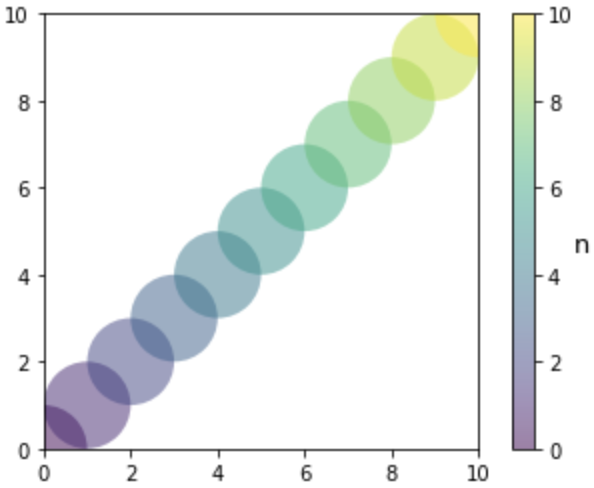
\includegraphics[width=0.43\columnwidth]{img/circles-n-n-1.png}
\end{wrapfigure}

Say we are using \tylr~ to edit a function that gets called by a
generative drawing application \cite{Processing,sns-pldi}.
The function takes an integer index and
returns a circle---represented as a pair comprising
its center point and radius---to be drawn in
the $xy$-plane for every index.
Shown above, the initial program draws unit circles
along the line $y = x$.

\subsection{Terms versus tiles}

\begin{figure}
  \centering

   \begin{subfigure}[c]{0.49\columnwidth}
      \centering
      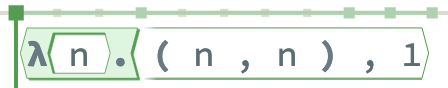
\includegraphics[width=0.9\textwidth]{img/pan-terms-0.png}
      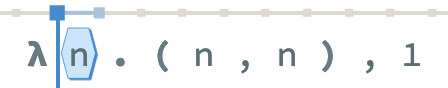
\includegraphics[width=0.9\textwidth]{img/pan-terms-1.png}
      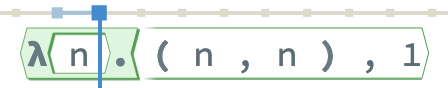
\includegraphics[width=0.9\textwidth]{img/pan-terms-2.png}
      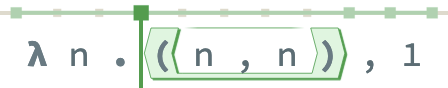
\includegraphics[width=0.9\textwidth]{img/pan-terms-3.png}
      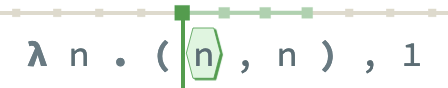
\includegraphics[width=0.9\textwidth]{img/pan-terms-4.png}
      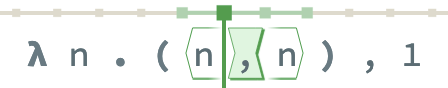
\includegraphics[width=0.9\textwidth]{img/pan-terms-5.png}
      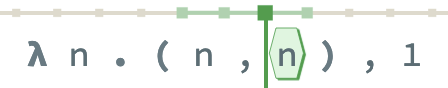
\includegraphics[width=0.9\textwidth]{img/pan-terms-6.png}
      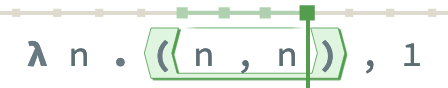
\includegraphics[width=0.9\textwidth]{img/pan-terms-7.png}
      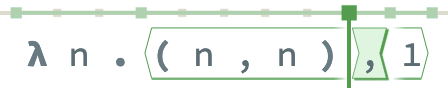
\includegraphics[width=0.9\textwidth]{img/pan-terms-8.png}
      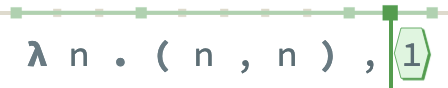
\includegraphics[width=0.9\textwidth]{img/pan-terms-9.png}
      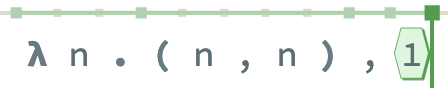
\includegraphics[width=0.9\textwidth]{img/pan-terms-10.png}
      \caption{}
      \label{fig:pan-term-view}
  \end{subfigure}
  \begin{subfigure}[c]{0.49\columnwidth}
    \centering
    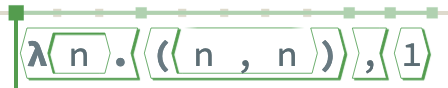
\includegraphics[width=0.9\textwidth]{img/pan-tiles-0.png}
    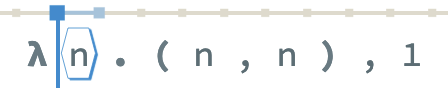
\includegraphics[width=0.9\textwidth]{img/pan-tiles-1.png}
    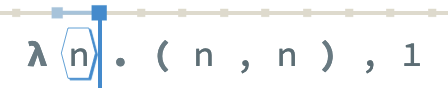
\includegraphics[width=0.9\textwidth]{img/pan-tiles-2.png}
    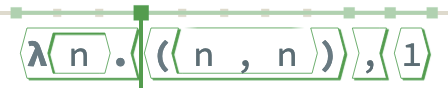
\includegraphics[width=0.9\textwidth]{img/pan-tiles-3.png}
    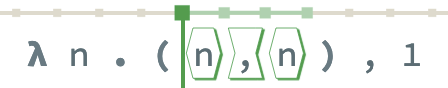
\includegraphics[width=0.9\textwidth]{img/pan-tiles-4.png}
    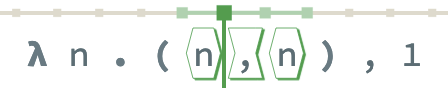
\includegraphics[width=0.9\textwidth]{img/pan-tiles-5.png}
    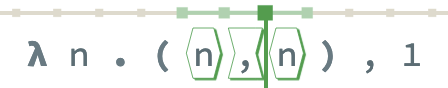
\includegraphics[width=0.9\textwidth]{img/pan-tiles-6.png}
    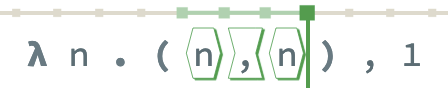
\includegraphics[width=0.9\textwidth]{img/pan-tiles-7.png}
    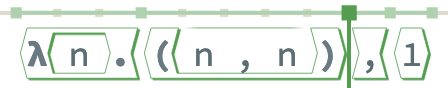
\includegraphics[width=0.9\textwidth]{img/pan-tiles-8.png}
    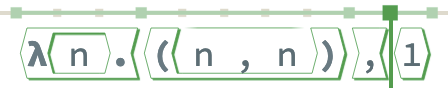
\includegraphics[width=0.9\textwidth]{img/pan-tiles-9.png}
    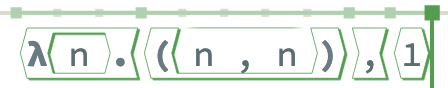
\includegraphics[width=0.9\textwidth]{img/pan-tiles-10.png}
    \caption{}
    \label{fig:pan-tile-view}
  \end{subfigure}
  \vspace{10pt}
  % \end{minipage}
  \caption{\tylr's pointing mode in \protect\subref{fig:pan-term-view} term view
  and \protect\subref{fig:pan-tile-view} tile view }
  \label{fig:pan}
\end{figure}

\begin{figure}
  \begin{subfigure}[c]{\columnwidth}
  \[
    \arraycolsep=3pt\begin{array}{rlrl}
        \text{pattern term} & \spat & ::= &
          \term{\ophole} ~\vert~
          \term{\svar{x}} ~\vert~
          \term{\sparen{\spat}} \\
        & & \vert &
          \term{\spat~\binhole~\spat} ~\vert~
          \term{\sprod{\spat}{\spat}} \\
        \text{expression term} & \sexp & ::= &
          \term{\ophole} ~\vert~
          \term{\snumlit{n}} ~\vert~
          \term{\svar{x}} ~\vert~
          \term{\sparen{\sexp}} \\
        & & \vert &
          % \sap{\sexp}{\sexp} ~\vert~
          \term{\sexp~\binhole~\sexp} ~\vert~
          \term{\sprod{\sexp}{\sexp}} \\
        & & \vert &
          \term{\splus{\sexp}{\sexp}} ~\vert~
          \term{\smult{\sexp}{\sexp}} ~\vert~
          \term{\sdiv{\sexp}{\sexp}} \\
        & & \vert &
          \term{\slam{\spat}{\sexp}} ~\vert~
          \term{\slet{\spat}{\sexp}{\sexp}}
    \end{array}\]
    \caption{}
    \label{fig:term-syntax}
  \end{subfigure}
  \vspace{0.4cm}

  \begin{subfigure}[c]{\columnwidth}
    \[\arraycolsep=3pt\begin{array}{rlrl}
      \text{tile sequence} & \tiles^s & ::= & \tile^s_1\dots\tile^s_n \\
      \text{pattern tile} & \tile^{\pat} & ::= &
        \tophole ~\vert~
        \soptile{\svar{x}} ~\vert~
        \soptile{\sparen{\tiles^{\pat}}} \\
      & & \vert &
        \tbinhole ~\vert~
        \sbintile{\tprod} \\
      \text{expression tile} & \tile^{\expr} & ::= &
        \tophole ~\vert~
        \soptile{\snumlit{n}} ~\vert~
        \soptile{\svar{x}} ~\vert~
        \soptile{\sparen{\tiles^{\expr}}} \\
      & & \vert &
        \tbinhole ~\vert~
        % \sap{}{} ~\vert~
        \sbintile{\tplus} ~\vert~
        \sbintile{\tmult} ~\vert~
        \sbintile{\tdiv} ~\vert~
        \sbintile{\tprod} \\
      & & \vert &
        \spretile{\tlam{\tiles^{\pat}}} ~\vert~
        \spretile{\tlet{\tiles^{\pat}}{\tiles^{\expr}}}
    \end{array}\]
    \caption{}
    \label{fig:tile-syntax}
  \end{subfigure}
  \vspace{0.4cm}
  \caption{
      Term syntax \protect\subref{fig:term-syntax} and tile syntax \protect\subref{fig:tile-syntax}
      for patterns and expressions,
      where
      $x$ ranges over variables
      % $b$ over boolean values,
      and $n$ over number literals.
  }
  \label{fig:term-tile-syntax}
\end{figure}

% \begin{figure}
  \vspace{-3px}
  \[\arraycolsep=3pt\begin{array}{rlrl}
    \text{tile sequence} & \tiles^s & ::= & \tile^s_1\dots\tile^s_n \\
    \text{pattern tile} & \tile^{\pat} & ::= &
      \ophole ~\vert~
      \svar{x} ~\vert~
      \sparen{\tiles^{\pat}} ~\vert~
      \binhole ~\vert~
      \sprod{}{} \\
    \text{expression tile} & \tile^{\expr} & ::= &
      \ophole ~\vert~
      \snumlit{n} ~\vert~
      \svar{x} ~\vert~
      \sparen{\tiles^{\expr}} \\
    & & \vert &
      \binhole ~\vert~
      % \sap{}{} ~\vert~
      \sprod{}{} ~\vert~
      \splus{}{} ~\vert~
      \smult{}{} \\
    & & \vert &
      \slam{\tiles^{\pat}}{} ~\vert~
      \slet{\tiles^{\pat}}{\tiles^{\expr}}{}
  \end{array}\]
  \caption{Tile syntax for patterns and expressions.}
  \label{fig:tile-syntax}
\end{figure}


% \note{maybe forward reference alternative choices not skipping tokens}
Panning the cursor over the program in \tylr,
as shown in Figure \ref{fig:pan-term-view},
reveals the program structure as
governed by \tylr's \emph{term syntax},
the relevant subset of which is shown in
Figure \ref{fig:term-syntax}.
For example, the first edit state in Figure \ref{fig:pan-term-view}
shows the top-level function---an expression term as
indicated by the green coloring---binding
the pattern variable \code{n} and returning an indexed circle.
Notice how every term has a convex hexagonal shape.

Highlighted within each term is a substructure called a \emph{tile};
with respect to the containing term, we say it is the term's \emph{root tile}.
Each term's root tile encompasses all root-level tokens used to
represent the term, along with children of the term that the tokens
delimit on both sides---such children we call \emph{bidelimited}.
For example, in the first edit state of
Figure \ref{fig:pan-term-view}, observe how the function's highlighted
tile spans the function's tokens \code{$\boldsymbol{\lambda}$}
and \code{\textbf{.}\vphantom{$\boldsymbol{\lambda}$}}
as well as the bidelimited pattern child; however, it does not
extend to the \emph{unidelimited} body child.

Holding Alt/Option while panning the cursor, this time in
Figure \ref{fig:pan-tile-view}, reveals the program structure
as governed by \tylr's \emph{tile syntax},
shown in Figure \ref{fig:tile-syntax}.
Tiles enjoy a flatter structure compared to the
strictly hierarchical terms.
Notice in the first edit state of Figure \ref{fig:pan-tile-view},
for example, how the tiles comprising the function body
are siblings with the function term's root tile.
The \emph{tips} of a tile indicate its syntactic
role in the tile sequence as a(n):
\toptile{operand}, \tpretile{prefix operator},
\tposttile{postfix operator}, or \tbintile{infix operator}.

Where traditional structure editors model their edit states
using the strictly hierarchical term syntax,
% \footnote{
%   Technically, most other structure editors model their edit states
%   in terms of the language's abstract syntax, whereas the
%   term syntax used here is more akin to the concrete syntax,
%   but the important point is that they are both strictly hierarchical.
% }
\tylr~ instead models its edit state using the flatter
tile syntax, precedence-parsing the tile structure
as needed to produce the term structure.
Indeed, the term structure shown in Figure \ref{fig:pan-term-view}
is simply a decoration overlaid atop the actual tile
structure shown in Figure \ref{fig:pan-tile-view}.
Moving forward, we will refer to structure editors
with term-structured edit states as \emph{term-based editors}.

\subsection{Opseqs \& holes}

The edit states shown in Figure \ref{fig:pan} are in
\emph{pointing mode}, \tylr's default editing mode.
Much like how a text editor's cursor points at positions
between characters in its default mode, \tylr's default
cursor points at positions between tiles.
% \note{note how they are explicitly indicated in above
% the terms/tiles, the local cursor positions for the current tile
% sequence are shown, that we can speak meaningfully of the
% sort of a cursor position, maybe forward reference that
% this will be useful for explaining how selecting works}
\tylr's central guarantee is: if you are in pointing mode,
then you have a well-formed program term.

Simply maintaining a well-formed tile structure
according to the tile syntax alone, however, is
not sufficient to uphold this guarantee.
The generic sequential structure of tile sequences
simplifies how we define edit operations, but
does not guarantee that the tiles represent a well-formed
\emph{operator sequence}, or \emph{opseq} for short.
The qualifications for a tile sequence to an opseq
enjoy a simple physical metaphor:
\begin{enumerate}
\item[(1)] every tile \emph{fits} its neighbors:
  if a pair of tips meet, they look like $\ltiletip\ltiletip$
  or $\rtiletip\rtiletip$; and
\item[(2)] every tile sequence is \emph{convex}:
  it is nonempty, the first tile's left tip $\ltiletip$
  points left, and the last tile's right tip $\rtiletip$
  points right.
\end{enumerate}
If \tylr~ maintains well-formed opseqs in pointing mode, then we have
our guarantee, since precedence-parsing is total on opseqs.

For this reason, \tylr~ automatically inserts
and removes placeholder tiles called \emph{holes}
as we edit to maintain opseq structure.
There are two kinds of holes:
\emph{operand holes} $\soptile{\ophole}$
and \emph{operator holes} $\sbintile{\binhole}$.
We will soon see a number of examples of
automatic hole fixing as we turn our attention
to editing.

% \note{also mention right bias of term view (for simplicity)}

% \note{following sentence too vague, couch in concrete example,
% be more clear about highlighting the root vs the whole tile,
% probably refer explicitly to tile syntax earlier to make it
% more precise}
% Highlighted at the root of every term is a structure called
% a \emph{tile}.
% The tile encompasses all tokens used to represent
% the root form of the term (e.g., \texttt{1} for a number literal,
% $\lambda$ and \texttt{.} for lambda terms,
% \texttt{(} and \texttt{)} for parenthesized terms) along with
% all children terms delimited on both sides (\eg,
% the bidelimited pattern child \texttt{n} of the lambda term,
% the bidelimited expression child \texttt{n , n} of
% the parenthesized term).

% Tiles are closely related to nested words \note{cite} and
% visibly pushdown languages \note{cite}, which we discuss
% further in Section \ref{sec:related-work}.

\subsection{Inserting and removing tiles} \label{sec:inserting-removing}
By having us edit the tile structure, and only
indirectly propagate those edits to the term structure,
\tylr~ recovers many of the flexible editing affordances to
which we are accustomed in text editors.

% \setlength\intextsep{0pt}
% \begin{wrapfigure}{r}{0.08\columnwidth}
%   \centering
%   \hspace*{-0.07\columnwidth}
%   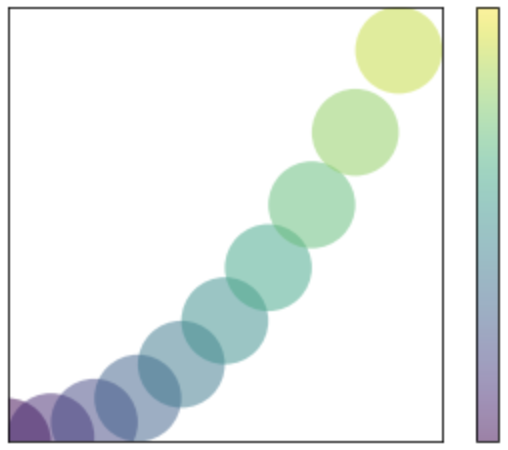
\includegraphics[width=0.15\columnwidth]{img/circles-parabola.png}
% \end{wrapfigure}

\paragraph{Leaf tiles}
We update the function to
draw circles along the parabola $y = x^2/9$,
% as depicted on the right,
using the edit sequence below.

\begin{center}
  \centering
% \begin{minipage}[t]{0.2\columnwidth}
%   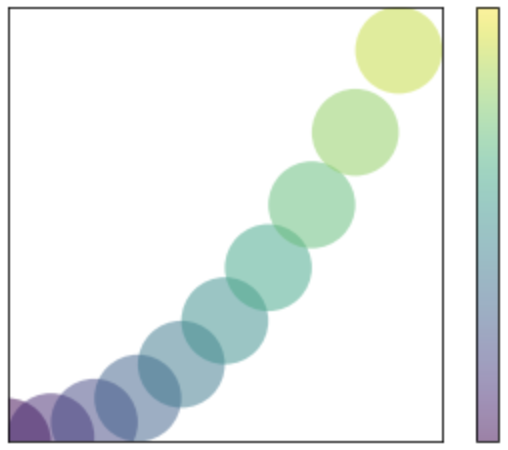
\includegraphics[width=\textwidth]{img/circles-parabola.png}
% \end{minipage}
% \hfill
% \begin{minipage}{0.65\columnwidth}
  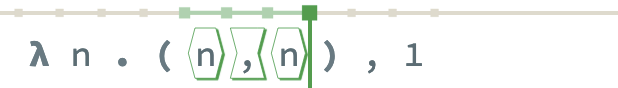
\includegraphics[width=0.6\columnwidth]{img/linear-insertion-0.png}
  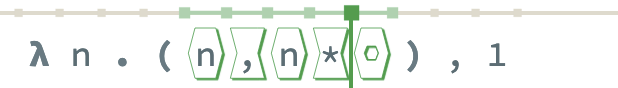
\includegraphics[width=0.6\columnwidth]{img/linear-insertion-1.png}
  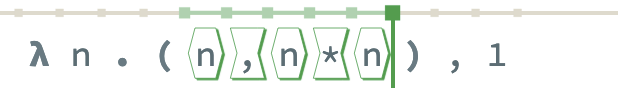
\includegraphics[width=0.6\columnwidth]{img/linear-insertion-2.png}
  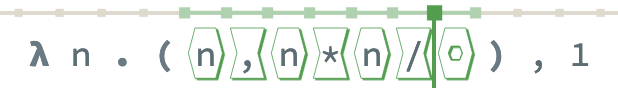
\includegraphics[width=0.6\columnwidth]{img/linear-insertion-3.png}
  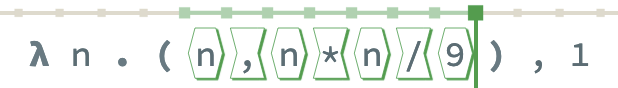
\includegraphics[width=0.6\columnwidth]{img/linear-insertion-4.png}
  % \caption{Inserting}
% \end{minipage}
\end{center}

% \setlength\intextsep{0pt}
% \begin{wrapfigure}{r}{0.08\columnwidth}
%   \centering
%   \hspace*{-0.07\columnwidth}
%   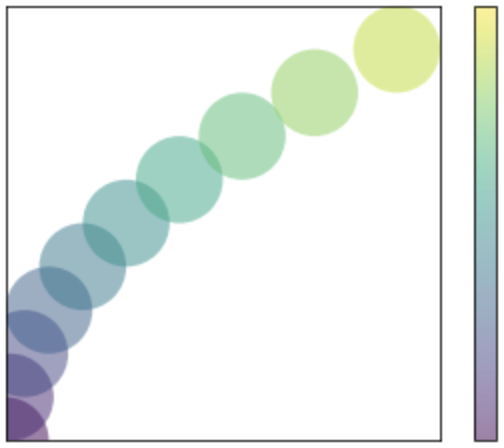
\includegraphics[width=0.15\columnwidth]{img/circles-parabola-transpose.png}
% \end{wrapfigure}

If we decided now to draw circles along the reflected
parabola $x = y^2/9$, we could similarly remove the inserted
tiles right-to-left from the $y$-coordinate and re-insert
them in the $x$-coordinate.

\begin{center}
  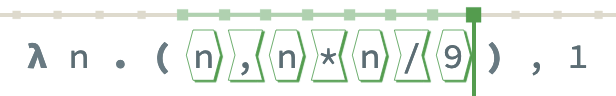
\includegraphics[width=0.6\columnwidth]{img/removal-0.png}
  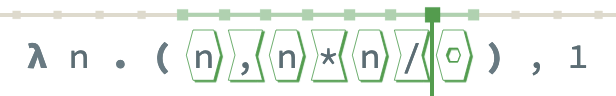
\includegraphics[width=0.6\columnwidth]{img/removal-1.png}
  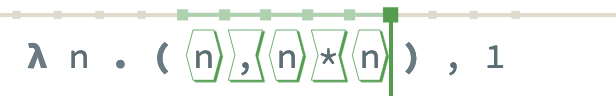
\includegraphics[width=0.6\columnwidth]{img/removal-2.png}
  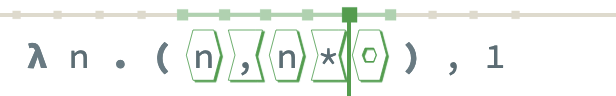
\includegraphics[width=0.6\columnwidth]{img/removal-3.png}
  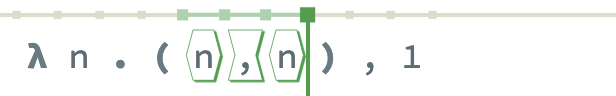
\includegraphics[width=0.6\columnwidth]{img/removal-4.png}
  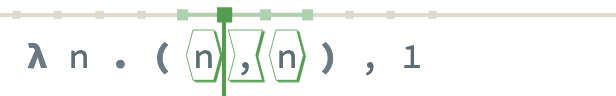
\includegraphics[width=0.6\columnwidth]{img/removal-5.png}
  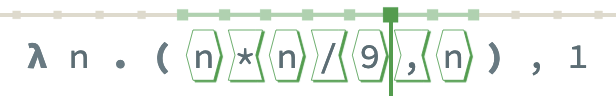
\includegraphics[width=0.6\columnwidth]{img/removal-6.png}
\end{center}

These simple editing workflows are not trivial
in traditional term-based editors because,
from the perspective of the AST, linear construction of
operator sequences is a complex, context-sensitive operation.
Existing structure editors either embrace strictly tree-based
construction of operator sequences \cite{scratch};
defer to text at the expression level \cite{Cornell,greenfoot},
recovering linearity at the cost of structure;
or solve the problem at the cost of complexity
\cite{GrammarCells}.
In contrast, tiles combined with automatic hole fixing
make it easy to define linear editing operations
without compromising structure.

% \note{add one more final snapshot in term view, showing
% how tylr parses precedence/associativity}

% \note{pause after constructing the times and note how
% precedence is re-parsed}

% \note{note that this is insertion, not ``hole filling'' as
% it is traditionally conceived in structure editors}

% \note{insert a comment somewhere about no performance claims}

% \note{review side transforms and make sure I'm not BSing}

% \note{figure out where to talk about hole insertion based on tips
% somewhere here}

% \tylr~ takes a different approach to this problem.
% Where traditional structure editors simply expose editing
% operations acting directly on the abstract syntactic struture
% of a program, \tylr~ presents the program in a separate
% concrete syntax with its own syntax-directed editing operations.
% \note{
%   talk about tile syntax show in Figure \ref{fig:tile-syntax},
%   note linearity
% }
% Like text, \tylr's concrete syntax gives you ``flattened''
% representation of your program that can be edited in a linear fashion.
% Unlike text, the concrete syntax maintains hierarchies of
% bidelimited children and can always be parsed into
% the abstract syntax, provided that the structure first undergoes
% a hole fixing pass in which holes are inserted and removed
% as needed. \note{need more context about tiles + bidelimited, bring
% back some old words about abstract syntactic structural units
% as opposed to concrete syntactic structural units}

% \note{perhaps go back to editor syntax terminology}

% \begin{figure*}
%   \begin{tabular}{cp{0.7\textwidth}}
%   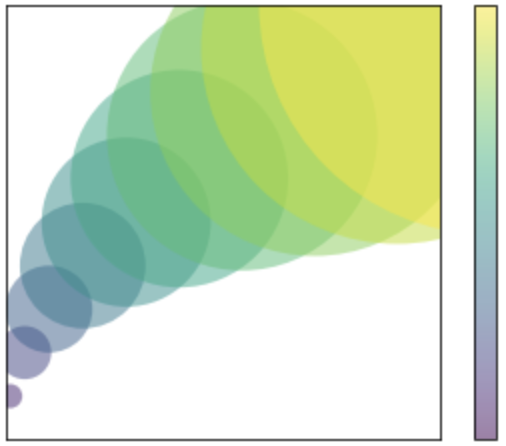
\includegraphics[width=0.1\textwidth]{img/circles-parabola-grow-1.png}
%   &
%   {
%     \begin{align*}
%       & \texttt{$\lambda$ n . let x , y = \_|in ( n * n / 9 , n ) , 1} \\
%       & \texttt{$\lambda$ n . let x , y = \_|in|( n * n / 9 , n ) , 1} \\
%       & \texttt{$\lambda$ n . let x , y = [in]( n * n / 9 , n ) , 1} \\
%       & \texttt{$\lambda$ n . let x , y = ( n * n / 9 , n )[in], 1} \\
%       & \texttt{$\lambda$ n . let x , y = ( n * n / 9 , n )|in \_ , 1} \\\\
%       & \texttt{$\lambda$ n . let x , y = ( n * n / 9 , n|) in x , y , 1 } \\
%       & \texttt{$\lambda$ n . let x , y = ( n * n / 9 , n|)|in x , y , 1 } \\
%       & \texttt{$\lambda$ n . let x , y = |(|n * n / 9 , n[)]in x , y , 1 } \\
%       & \texttt{$\lambda$ n . let x , y = |(|[)]n * n / 9 , n in x , y , 1 } \\
%       & \texttt{$\lambda$ n . let x , y = [(][)]n * n / 9 , n in x , y , 1 } \\
%       & \texttt{$\lambda$ n . let x , y = n * n / 9 , n in [(][)]x , y , 1 } \\
%       & \texttt{$\lambda$ n . let x , y = n * n / 9 , n in ( x , y[)], 1 } \\
%       & \texttt{$\lambda$ n . let x , y = n * n / 9 , n in ( x , y|) , 1 } \\\\
%       & \texttt{$\lambda$ n . let x , y = n * n / 9 , n in ( x , y ) ,|x + y } \\
%       & \texttt{$\lambda$ n . let x , y = n * n / 9 , n in ( x , y ) ,|(|[)]x + y } \\
%       & \texttt{$\lambda$ n . let x , y = n * n / 9 , n in ( x , y ) ,|(|x + y[)]} \\
%       & \texttt{$\lambda$ n . let x , y = n * n / 9 , n in ( x , y ) , ( x + y|)} \\
%       & \texttt{$\lambda$ n . let x , y = n * n / 9 , n in ( x , y ) , ( x + y )|} \\
%       & \texttt{$\lambda$ n . let x , y = n * n / 9 , n in ( x , y ) , ( x + y ) /|\_} \\
%       & \texttt{$\lambda$ n . let x , y = n * n / 9 , n in ( x , y ) , ( x + y ) / 4|}
%     \end{align*}
%   }
%   \end{tabular}
% \end{figure*}

% \begin{figure*}
%   \begin{tabular}{cp{0.7\textwidth}}
%   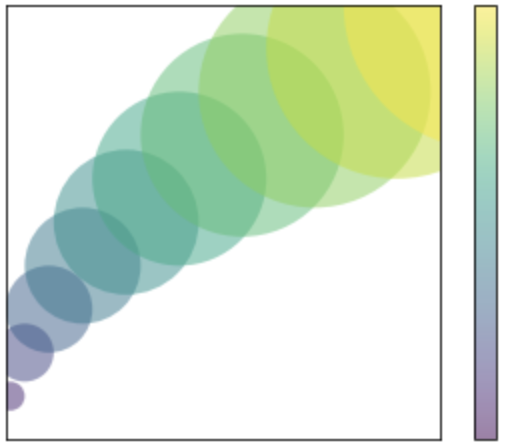
\includegraphics[width=0.1\textwidth]{img/circles-parabola-grow-2.png}
%   &
%   {
%     \begin{align*}
%       & \texttt{$\lambda$ n . let x , y = n * n / 9 , n|in ( x , y ) , n / 3} \\
%       & \texttt{$\lambda$ n .|let x , y =|n * n / 9 , n[in] ( x , y ) , n / 3} \\
%       & \texttt{$\lambda$ n . n * n / 9 , n|\_ ( x , y ) , n / 3} \\
%       & \texttt{$\lambda$ n . n * n / 9 , n \_ (|x , y ) , n / 3} \\
%       & \texttt{$\lambda$ n . n * n / 9 , n \_ (|x , y|) , n / 3} \\
%       & \texttt{$\lambda$ n . n * n / 9 , n \_ (|\_ ) , n / 3} \\
%       & \texttt{$\lambda$ n . n * n / 9 , n [(]|)|, n / 3} \\
%       & \texttt{$\lambda$ n .[(]n * n / 9 , n|)|, n / 3} \\
%       & \texttt{$\lambda$ n .|( n * n / 9 , n ), n / 3}
%     \end{align*}
%   }
%   \end{tabular}
% \end{figure*}

\paragraph{Non-leaf tiles}
While insertion and removal of leaf tiles closely mimics the
text editing experience, this begins to change as we turn our
attention to non-leaf tiles.
For example, consider below how we would remove the parentheses
wrapping the origin coordinates in \tylr.

\begin{center}
  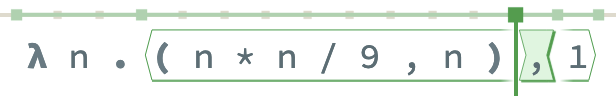
\includegraphics[width=0.6\columnwidth]{img/remove-nonleaf-0.png}
  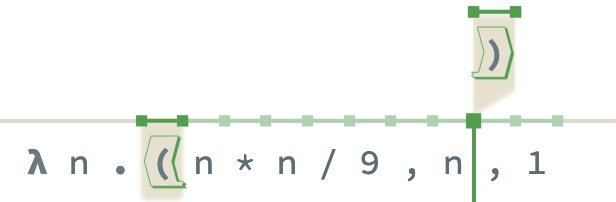
\includegraphics[width=0.6\columnwidth]{img/remove-nonleaf-1.png}
  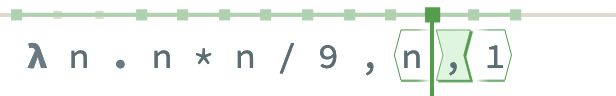
\includegraphics[width=0.6\columnwidth]{img/remove-nonleaf-2.png}
\end{center}

Where a text editor would simply remove the closing parenthesis
on the first Backspace, leaving us with a syntax error,
\tylr~ first enters an intermediate state in which it has
"picked up" the closing parenthesis and highlighted the
matching opening parenthesis.
Pressing Backspace again then removes both parentheses.

This intermediate state is called \emph{restructuring mode},
and we picked up the closing parenthesis into the \emph{backpack};
we will soon discuss these at greater length.
For now, notice how restructuring mode served as a
sort of confirmation dialog, showing us that removing
the token on which we hit Backspace would require
deleting other tokens.
We believe such explicit confirmation is important to
prevent ``spooky action at a distance'', especially
in light of the MPS user data discussed in Section \ref{sec:intro}.

Now consider how we might re-insert the parentheses
around the origin coordinates.

\begin{center}
  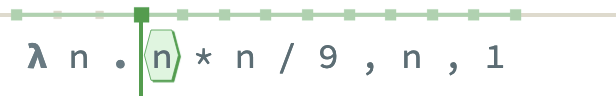
\includegraphics[width=0.6\columnwidth]{img/insert-nonleaf-0.png}
  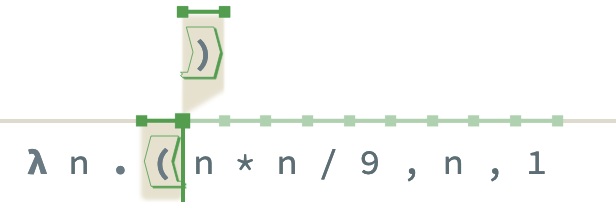
\includegraphics[width=0.6\columnwidth]{img/insert-nonleaf-1.png}
  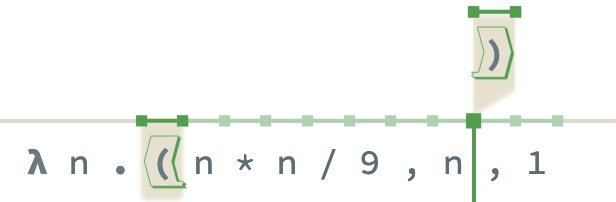
\includegraphics[width=0.6\columnwidth]{img/insert-nonleaf-2.png}
  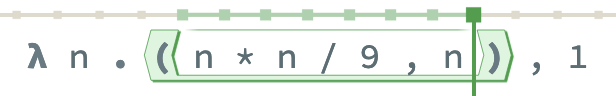
\includegraphics[width=0.6\columnwidth]{img/insert-nonleaf-3.png}
\end{center}

\noindent
In a dual fashion to removal, inserting
an opening parenthesis enters restructuring mode with its
matching closing parenthesis in the backpack.
Restructuring mode then allows us to move the parenthesis
to the right and put it down.
Notice the similarity to the text editing experience,
which has an invoke-then-configure flow, whereas a typical
structure editor would require you to select the body before
parenthesizing, forcing preemptive configuration before
invocation.

MPS supports a similar editing flow for parentheses in particular,
but not any other syntactic forms also with matching delimiters.
In contrast, as we will see next, \tylr~ has well-defined
restructuring behavior for arbitrary range selections.

\subsection{Selecting and restructuring} \label{sec:selecting-restructuring}

Using the arrow keys while holding
Shift enters \tylr's \emph{selecting mode}.

\noindent
\begin{minipage}[t]{0.495\columnwidth}
  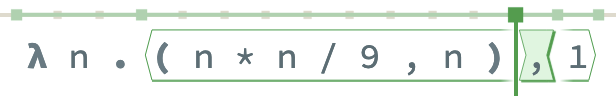
\includegraphics[width=\textwidth]{img/selection-0.png}
  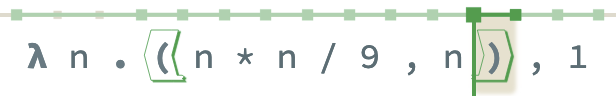
\includegraphics[width=\textwidth]{img/selection-1.png}
  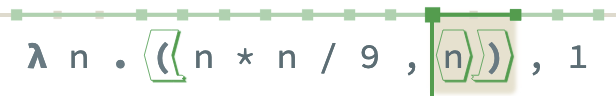
\includegraphics[width=\textwidth]{img/selection-2.png}
  \includegraphics[width=\textwidth]{img/selection-3.png}
  \includegraphics[width=\textwidth]{img/selection-4.png}
\end{minipage}
\hfill
\begin{minipage}[t]{0.495\columnwidth}
  \includegraphics[width=\textwidth]{img/selection-5.png}
  \includegraphics[width=\textwidth]{img/selection-6.png}
  \includegraphics[width=\textwidth]{img/selection-7.png}
  \includegraphics[width=\textwidth]{img/selection-8.png}
  \includegraphics[width=\textwidth]{img/selection-9.png}
\end{minipage}

\noindent
Selecting mode lets us specify arbitrary range selections up
to token boundaries.
Notice how, when a tile is divided by a selection boundary,
it is disassembled into individual \emph{shards}.
Then, once they are all within or without the selection,
the shards are reassembled into the original tile.

Collectively we call tiles and shards \emph{pieces},
a sequence of pieces a \emph{segment}.
A segment containing only tiles is called \emph{intact},
otherwise \emph{cracked}.
We may understand restructuring mode, not simply as a tile insertion
and removal aid, but more generally as a structured variant of
cut-and-paste of selected segments, regulated by their intact versus
cracked structure.

% Tiles not only simplify linear \emph{insertion} in a structured
% context but also enable text-like \emph{selecting}
% and \emph{restructuring} (e.g. cut and paste) of existing code.
% While the former problem is relatively well-studied
% \note{cite MPS, modeless structure editing},
% almost no attention has been paid to the latter.
% In particular, all prior structure editors restrict
% structured selections to complete concrete syntactic terms,
% a severe limitation compared to the arbitrary range
% selections of text editors.

% \tylr~ recovers much of this lost flexibility.
% Using \tylr's \emph{selecting mode}, you can
% make arbitrary range selections up to token boundaries,
% disassembling tiles into \emph{shards} as needed.
% Using \tylr's \emph{restructuring mode},
% you can pick up your selections into your
% \emph{backpack} and put them down elsewhere,
% à la cut-and-paste using the clipboard.
% Unlike the usual clipboard, however,
% your backpack is structure-aware and guides your
% movement toward valid paste targets, \ie,
% you can only put down your backpack's contents
% where the result can be reassembled into well-formed tiles.

% \note{add another paragraph header focused on selecting}

% \note{see if I can talk about intact vs cracked selections here,
% perhaps by changing the direction of the first selection and
% introducing shards when right parens get selected}

% \note{so far we have been in pointing mode...}

% \setlength\intextsep{0pt}
% \begin{wrapfigure}{r}{0.08\columnwidth}
%   \centering
%   \hspace*{-0.07\columnwidth}
%   \includegraphics[width=0.15\columnwidth]{img/circles-parabola-transpose.png}
% \end{wrapfigure}

\paragraph{Restructuring with a full backpack}
In Section \ref{sec:inserting-removing}, we updated the circle drawing tracing the
parabola $y = x^2/9$ to its reflection $x = y^2/9$ by deleting
and re-inserting tiles.
Alternatively, we could have selected the inserted tiles---an impossible
selection in a term-based editor---and used
restructuring mode to move them.
% Say you update your circle drawing
% to its transposition, i.e., draw the circles along
% the parabola $x = y^2/9$.
% Entering selecting mode, you anchor the selection's right
% end and move left to select the tiles you just
% inserted in the $y$-coordinate---an impossible
% selection in prior structure editors.

\begin{center}
  \includegraphics[width=0.6\columnwidth]{img/restructuring-full-0.png}
  \includegraphics[width=0.6\columnwidth]{img/restructuring-full-1.png}
  \includegraphics[width=0.6\columnwidth]{img/restructuring-full-2.png}
  \includegraphics[width=0.6\columnwidth]{img/restructuring-full-3.png}
  \includegraphics[width=0.6\columnwidth]{img/restructuring-full-4.png}
\end{center}
% You then pick it up into your backpack to enter
% restructuring mode.
% Moving left to the $x$-coordinate and putting down
% the selection completes the desired transformation.

% \noindent
% \begin{tabular}{cp{7cm}}
% \includegraphics[width=2cm]{img/circles-parabola-transpose.png}
% &
% {
% \begin{align*}
%   & \texttt{$\lambda$ n . ( n , n[* n / 9]) , 1} \\
%   & \texttt{$\lambda$ n . ( n ,[* n / 9]n ) , 1} \\
%   & \texttt{$\lambda$ n . ( n[* n / 9], n ) , 1} \\
%   & \texttt{$\lambda$ n . ( n|* n / 9 , n ) , 1}
% \end{align*}
% }
% \end{tabular}

% \note{define intact selections}

We say that the backpack is \emph{full} whenever
its contents are, or could be assembled into, an intact selection.
If the backpack is full, then we may move freely,
since we may insert a selection of whole tiles anywhere
without compromising the existing shard-balanced structure.

% \note{define cracked selections}

Often, however, the backpack's contents are not an intact
selection, nor can they be assembled into one, as we observed
in the parentheses insertion and removal examples in Section \ref{sec:inserting-removing}.
In that case, we say that the backpack is \emph{hungry}...

\paragraph{Restructuring with a hungry backpack}

Now we would like the circles' radii to grow
with their origin coordinates; accordingly,
as shown at the top of the edit sequence below,
we have inserted
a let tile introducing variables \code{x} and \code{y}
in the function body.
Our next task is to restructure our code so that \code{x}
and \code{y} are bound to the origin coordinates
\code{( n * n / 9 , n )} currently in the body of the let term.
We select the \code{in} delimiter,
disassembling the \code{let}-tile in the process;
move right once; and put it down,
upon which \tylr~ reassembles the \code{let}-tile
and returns us to pointing mode.

\begin{center}
  \includegraphics[width=\columnwidth]{img/restructure-hungry-0.png}
  \includegraphics[width=\columnwidth]{img/restructure-hungry-1.png}
  \includegraphics[width=\columnwidth]{img/restructure-hungry-2.png}
  \includegraphics[width=\columnwidth]{img/restructure-hungry-3.png}
  \includegraphics[width=\columnwidth]{img/restructure-hungry-4.png}
\end{center}

% \note{figure out a way to introduce hole fixing, why operand hole
% disappears rather than operator hole being introduced, might be
% here or worked in before}

% \note{when discussing hole minimality, distinguish from other
% interfaces where you insert holes manually, so you shouldn't
% remove automatically}

% Your editing workflow was similar to what you might
% have done in a text editor---delete the \texttt{in}
% delimiter, move right, re-type---except that \tylr~
% skipped all cursor positions within the parentheses tile
% when you moved right.
Notice that we skipped all cursor positions within
the parentheses tile when we moved right.
The \code{in}-shard in our backpack could not be assembled into
a whole tile on its own, meaning at least one matching shard---in
this case, \code{let x , y =}---was
anchored within the current tile sequence.
This restricted our movement of the \texttt{in}-shard
to cursor positions of the same sequence,
as placing it in any other position would
violate proper nesting of matching shards.

% \note{add back some discussion comparing to text editing
% and other structure editors;
% similarity with text workflow,
% while making it more efficient + less cognitive load;
% other structure editors would force you to translate
% edits into term-based selections, can be awkward or
% not the most efficient in terms of selection size}

We call the backpack full or hungry as a way
to narrativize its control of our movement.
When the backpack is full, it is satisfied
and lets us move freely and leisurely through
our code.
When the backpack is hungry, it accelerates our
movement through the current tile sequence
in its impatience to end its hunger, which can happen in one of two ways.
Either, like in the last example, we can empty the backpack,
freeing it of all earthly possessions and desires;
or we may feed it.

% \note{add forward reference to discussing alternatives, eg,
% not skipping cursor positions}

% We hypothesize that such a restriction would lead to both greater
% editing efficiency and reduced cognitive load compared to
% text editing on similar tasks.

% We hypothesize that such a restriction would easy to learn
% given
% \begin{itemize}
% \item be easy to learn, given the workflow similarity to text editing;
% \item lead to greater editing efficiency than text editing due to
%     the fewer keypresses needed to reach valid paste/restructure targets; and
% \item reduce cognitive load compared to text editing because you
%     no longer need to count delimiters to ensure you have reached
%     a valid paste/restructure target.
% \end{itemize}

\paragraph{Feeding a hungry backpack}
Say we have rewritten the origin in terms of
\code{x} and \code{y}, as shown at the top of the
edit sequence below.
Along the way, however, we forgot to parenthesize
the origin coordinates.
We also notice that the parentheses in the definition
of the \code{let}-tile are now redundant and decide
to recycle them.
\begin{center}
  \includegraphics[width=\columnwidth]{img/multi-restructure-0.png}
  \includegraphics[width=\columnwidth]{img/multi-restructure-1.png}
  \includegraphics[width=\columnwidth]{img/multi-restructure-2.png}
\end{center}
At this point the backpack is hungry and restricts
our movement to the tile sequence within the
let definition.
Instead of emptying our backpack like in the
last example, this time we move over to the
left parenthesis and pick it up as well.
\begin{center}
  \includegraphics[width=\columnwidth]{img/multi-restructure-3.png}
  \includegraphics[width=\columnwidth]{img/multi-restructure-4.png}
\end{center}
Now our backpack is full, as it carries both shards
needed to assemble a parentheses tile, and we may
now move freely out of the let definition
to put down the parentheses around the origin coordinates.
\begin{center}
  \includegraphics[width=\columnwidth]{img/multi-restructure-5.png}
  \includegraphics[width=\columnwidth]{img/multi-restructure-6.png}
  \includegraphics[width=\columnwidth]{img/multi-restructure-7.png}
  \includegraphics[width=\columnwidth]{img/multi-restructure-8.png}
  \includegraphics[width=\columnwidth]{img/multi-restructure-9.png}
\end{center}

The last example showed how \tylr~ lets us carry \emph{multiple}
related range selections in the backpack.
This ability significantly improves our selecting precision
compared to prior designs.
From the perspective of the term syntax,
where other structure editors force us to select
complete subtrees, \tylr~ lets us cut out individual
\emph{nodes} of the tree and splice them back in
elsewhere.

% \note{add labels to edit states,
% label sentences here}

% Say you have filled the hole in Figure ?? with
% the variables \texttt{x} and \texttt{y} you defined
% in the previous example, as shown in Figure ??.
% Upon reviewing the term structure, however, you
% discover that pairs are right-associative in \tylr,
% so you need to wrap \texttt{x , y} in parentheses
% in order to satisfy the expected return type.
% \note{maybe just say we've created a triple but we
% really want a pair of a pair on left}
% You also notice that the parentheses in the definition
% of the \texttt{let} tile are now redundant
% and decide to recycle them.
% You move your cursor to the right parenthesis,
% select it, and pick it up into your backpack.
% At this point your backpack is hungry and restricts
% your movement to the tile sequence within the
% let definition.
% Instead of emptying your backpack like in the
% last example, this time you move over to the
% left parenthesis and pick it up as well (Figure ??).

% \note{make note of pattern not having parentheses}

% When your backpack carries multiple selections,
% it dictates the order in which you can put them down.
% Most of the time it behaves like a stack, putting
% down first the last picked up selection; we discuss
% deviations

% Now your backpack is full, as it carries both shards
% needed to assemble a whole parentheses tile,
% and you may move freely again.
% You carry the parentheses over to the body of the
% let term and wrap \texttt{x , y} to complete your
% restructuring.

% \note{either remove this or rewrite when it's more as
% an emergent phenomenon}

% \paragraph{Staging tile insertion}
% \note{maybe just call restructuring on insertion}

% \note{add connecting intro connecting to node-centric perspective}
% Say you have completed an initial draft of your goal program,
% where each circle's radius is the sum of its origin
% coordinates, as shown in Figure ??.
% You discover, however, that the circles are so large that
% they fill your viewport, so you would like to make them smaller.
% You begin by inserting a left parenthesis
% before \texttt{x + y}, your intention being to wrap
% the sum and divide it by a constant factor.
% Upon this insertion, \tylr~ automatically enters
% restructuring mode with the matching right parenthesis
% in your backpack.
% You move right, put down the right parenthesis,
% and complete your desired transformation.

% \note{add discussion}

% \note{note how other structure editors force you to select
% child first before constructing}

\paragraph{Picky eating}
Not all selections can be picked up.
We call the cursor positions marking the ends of a selection
the selection's \emph{caps}.
So far we have only encountered selections with caps
of the same sort.
Your backpack is a picky eater in that
it will refuse to carry any selections with caps of
different sort.

Consider, for example, the following selection:

\begin{center}
  \includegraphics[width=\columnwidth]{img/broken-overline.png}
\end{center}


\noindent
The left cap is pattern-sorted while the right cap
is expression-sorted, as indicated by the two-toned
broken overline.
Picking up this selection would bring together
tiles of different sort, violating \tylr's edit
state well-formedness, so you are prevented from doing so.

% \note{show small inline example of selecting
% selection with caps of different sort}

% \note{show small inline example of selection
% with pattern caps cutting across expressions}

\subsection{Removing selections}

Lastly, we turn our attention to selection removal,
generalizing our understanding of tile removal
in pointing mode as discussed in
Section \ref{sec:inserting-removing}.
% Pressing Backspace on a selection
% has one of two effects:
% (1) if it is intact, remove the selection
%     and return to pointing mode;
% (2) otherwise, enter restructuring mode with
%     the smallest containing same-sort-capped selection
%     in your backpack.
% Pressing Backspace again in restructuring mode
% removes all highlighted tiles and selections.
Removing a selection works in one of two ways,
depending on whether the selection is intact or cracked.

\paragraph{Removing intact selections}
Say we fiddled around with different ways to make
the circles' radii grow.
Upon reviewing our code, we realize we no longer
need to define variables \code{x} and \code{y},
since they are each used only once, and can inline
their definition.
We begin by removing the uses of \code{x} and \code{y},
selecting \code{x , y} in the body of the \code{let}
term and hitting Backspace.
In this case, because our selection is intact, \tylr~
immediately removes our selection, as we might
expect from our experience with text editors.
\begin{center}
  \includegraphics[width=\columnwidth]{img/remove-intact-0.png}
  \includegraphics[width=\columnwidth]{img/remove-intact-1.png}
  \includegraphics[width=\columnwidth]{img/remove-intact-2.png}
\end{center}

\paragraph{Removing cracked selections}
Now we would like to remove the \code{let}-tile,
but we want to preserve its definition so we
can inline it.
We select the \code{in}-shard and hit Backspace.
Because our selection is cracked, removing
our selection would require also removing the
matching \code{let}-shard that we have not
explicitly selected ourselves.
\begin{center}
  \includegraphics[width=0.9\columnwidth]{img/remove-cracked-0.png}
  \includegraphics[width=0.9\columnwidth]{img/remove-cracked-1.png}
  \includegraphics[width=0.9\columnwidth]{img/remove-cracked-2.png}
  \includegraphics[width=0.9\columnwidth]{img/remove-cracked-3.png}
\end{center}
\tylr~ does not remove both shards immediately but
instead enters restructuring mode, giving us the option
to move the \code{in}-shard like in Section \ref{sec:selecting-restructuring},
or to proceed with removal of the highlighted pieces
like in Section \ref{sec:inserting-removing}.
We confirm the total removal by hitting Backspace again,
leaving behind the let definition and body
separated by an operator hole.

% In general, pressing Backspace on a selection
% has one of two effects:
% \begin{enumerate}
%   \item[(1)] remove the selection if it is intact
%     and return to pointing mode;
%   \item[(2)] otherwise entering restructuring mode with
%     the smallest containing selection with same-sort caps
%     in your backpack.
% \end{enumerate}
% Pressing Backspace again in restructuring mode
% removes all highlighted tiles and selections.
% In sum: if your selection is intact then you can
% remove it with a single tap of Backspace; otherwise
% you need to double tap.

% If your selection is fragmentary, then removing
% your selection would require also removing matching shards
% that you have not explicitly selected yourself.
% \tylr~ does not remove the implicit selections immediately
% but instead enters restructuring mode as a staging
% ground in which you may confirm the total removal
% by hitting Backspace again (or otherwise proceed
% with restructuring).
% \note{draw parallel with staged insertion}
% In sum: if your selection is intact then you can
% remove it with a single tap of Backspace; otherwise
% you need to double tap.


\paragraph{Removing in pointing mode}
Finally, it remains to restructure the parentheses
so that they wrap the origin coordinates.
This time, instead of first explicitly specifying a selection,
we position our cursor after the left parenthesis
and hit Backspace within pointing mode.
\tylr~ treats this input simply as a shortcut for selecting the
token immediately to our left and then hitting Backspace.
In this case, the token to our left is a parenthesis
shard that forms a cracked selection, so we
enter restructuring mode with the parenthesis in tow.
We move left to the other side of the origin coordinates,
then put down the parenthesis to complete the transformation.
\begin{center}
  \includegraphics[width=0.6\columnwidth]{img/remove-pointing-0.png}
  \includegraphics[width=0.6\columnwidth]{img/remove-pointing-1.png}
  \includegraphics[width=0.6\columnwidth]{img/remove-pointing-2.png}
  \includegraphics[width=0.6\columnwidth]{img/remove-pointing-3.png}
\end{center}

% \note{more words here to wrap up}


%\note{consider doing insertion, selection, deletion, then
%restructuring as a better progression}


% \subsection{\note{everything below this is old overview}}

% Tile-based structure editing departs from traditional
% structure editors in avoiding direct user modifications
% to the AST.
% Instead, much like with a text editor, the user modifies a separate
% ``flattened'' editing structure that affords more flexible
% editing mechanisms, which is subsequently parsed into the
% abstract syntax.
% Unlike a text editor, however, a tile-based editor ensures
% that every edit state can be parsed successfully.

% In this section we motivate and give an example-driven
% overview of tile-based editing as implemented
% in \tylr. We begin by describing the limitations of
% traditional structure editors, then show how tile-based
% editing overcomes these limitations.

% \subsection{A typical structure editor} \label{sec:simple-editor}

% Structure editors, also known as projectional editors, typically
% follow a projectional architecture: the editor projects an
% abstract syntax tree into a concrete representation,
% and user interactions with the representation are interpreted
% by the editor as direct modifications to the AST.

% For example, suppose we wish to edit expressions with the abstract
% syntax presented in Figure \ref{fig:tile-syntax}.
% A simple editor might project the current expression
% to a textual notation decorated with nested boxes, such
% that there is a one-to-one correspondence between
% boxes and terms. \note{example}
% In this editor, the cursor selects a subterm of the
% current program expression and may be moved through
% the current expression via a pre-order traversal.
% Edits are context-free transformations
% of the selected subterm:
%   deletion replaces the current subterm with
%     a hole of the same sort; and
%   construction replaces the current subterm
%     with the new form, making the original subterm
%     a child of the new form if possible, and moving
%     the cursor to the next child position if available.

% While simple, this editor is representative of existing structure
% editors in the way that it restricts editing affordances to easily
% understood tree manipulations of the abstract syntax.
% We believe such restrictions unacceptably hamper usability.
% Consider the following classes of edits that we may wish to
% perform---and could perform in a text editor---but cannot with the
% given interface:

% \paragraph{Linearly constructing operator sequences}
% In a text editor, we may type the characters \texttt{2}, \texttt{*},
% \texttt{3}, \texttt{+}, \texttt{4}
% to construct the expression \texttt{2 * 3 + 4} with
% the usual precedence-based operator associations.
% In our simple structure editor, the same inputs would construct
% the following series of edit states: \note{todo figure}.
% To get the associations we want, we would need to interleave
% our constructions with movements through the expression tree
% to ensure that the correct child is chosen before constructing
% the plus node: \note{todo figure}.
% This particular limitation of structure editing is well-recognized
% in prior work, which we discuss in greater detail in Section
% \ref{sec:related-work}.

% \paragraph{Preserving children of deleted terms}
% Deletion in our simple editor is quite coarse, deleting whole
% trees rather than individual nodes.


% \begin{itemize}
% \item
%   we now describe a few classes of edits that we may wish to perform---and
%   could perform in a text editor---but cannot with the given structured
%   interface
% \item structure-oblivious linear construction of operator sequences
%   \begin{itemize}
%     \item eg going from \texttt{2 * 3 + 4} as opposed to \texttt{2 * (3 + 4)}
%     \item this particular limitation of naive structure editing has received
%       the most attention in prior work
%     \begin{itemize}
%       \item some structure editors defer to text at the leaves
%       \item others develop more sophisticated methods, e.g.,
%         modeless structure editing article,
%         MPS's side transforms
%     \end{itemize}
%   \end{itemize}
% \item deleting the root of a term,
%   leaving behind its children for further processing
%   (eg splicing into the surrounding context)
%   \begin{itemize}
%     \item eg it is not possible to delete a let expression and leave behind its body
%     \item eg it is not possible to remove a conditional expression
%       and leave behind a branch to take its place, or to subsequently join the
%       two remaining branches with an operator
%     \item note how there's no room in the strict tree structure to deal with
%       multiple "floating" children
%     \item MPS mitigates this by leaving behind its first child if its the
%       same sort, but already this does not satisfy the use case described above,
%       and in general the user should have the freedom to choose
%   \end{itemize}
% \item selecting and restructuring sub- and cross-structural
%   parts of the program
%   \begin{itemize}
%     \item eg it is not possible to select \texttt{3 + 4} in \texttt{2 * 3 + 4}
%       and re-associate the expression, as one might in a text editor by
%       wrapping the selection in parentheses
%     \item eg it is not possible to select \texttt{let x = \_ in} and
%       move it before \texttt{let y = 2 in}
%     \item eg it is not possible to select \texttt{in} of \texttt{let x = \_ in}
%       and move it to wrap the subsequent portion of the expression
%     \begin{itemize}
%       \item as one might in a text editor by deleting \texttt{in},
%         moving the caret, re-typing it elsewhere
%       \item as one might when constructing the let line for the first time:
%         having typed out \texttt{let x =}, it remains to move the caret over
%         and type the \texttt{in}
%     \end{itemize}
%     \item while some of these examples are contrived given the simplicity of
%       the language, such selections and edits occur frequently in practice
%     \begin{itemize}
%       \item eg 6\% of logged edits in Design Requirements
%         paper involve making
%         selections across structural boundaries, 10\% of edits excluding those
%         that only involve name changes rather than structural changes
%     \end{itemize}
%   \end{itemize}
% \end{itemize}

% \subsection{\tylr: a tile-based editor}

% We now describe the design of \tylr, a tile-based structure
% editor.
% Given the disadvantages of operating directly on abstract syntax
% trees, \tylr~ presents programs to the user in a separate
% concrete syntax equipped with its own syntax-directed editing
% mechanisms.
% The concrete syntax is a ``flattened'' version of the abstract
% syntax, where the structural units correspond not to semantic
% terms of the language but rather syntactic groups of matching
% delimiters and their bidelimited children.
% We call these structural units \emph{tiles}.
% Figure \ref{fig:tile-syntax} shows the subset of \tylr's
% concrete syntax corresponding to the abstract syntax in
% Figure \ref{fig:language-syntax}.

% Unlike terms of the abstract syntax, tiles can be arranged
% sequentially.
% The cursor resides between consecutive pairs of
% tiles (or between a tile and its parent container),
% much as a text cursor resides between characters.
% Figure \note{todo} shows the different cursor positions
% in the operator sequence \texttt{2 * 3 + 4}.

% \subsubsection{Linear construction of operator sequences}
% Figure \note{todo} shows the construction of the operator
% sequence \texttt{2 * 3 + 4}. Unlike with the simple editor described
% in Section \ref{sec:simple-editor}, it is not necessary

% Unlike terms in the abstract syntax, tiles may be arranged
% sequentially as well as hierarchically.

% Rather than manipulating structures of the language syntax,
% a tile-based structure editor works within a parallel editor syntax.
% The central form in the editor syntax is the unassociated operator
% sequence. Operator sequence elements each take one of four shapes---operand,
% unary prefix, unary postfix, and
% binary infix---which we collectively refer to as \emph{tiles}.
% Tiles may in turn contain nested operator sequences.

% Like text, the editor syntax provides a flattened, more linear representation
% of the language syntax.
% Unlike text, the editor syntax maintains hierarchies of
% bidelimited children and can always be parsed into the
% language syntax, provided that the structure first undergoes
% a hole fixing pass in which holes are inserted and removed
% as needed.

% \note{talk about automatic hole fixing + operand vs operator holes}

% \note{after describing, note bonus edits that combine limitations from previous selection}

% \note{do get into how restructuring mode fits naturally within the deletion vs construction}